\chapter{Odpowied� skokowa dla algorytmu DMC}

\section{Odpowied� skokowa}
Do wyznaczania odpowiedzi skokowej dla algorytmu DMC wybrana zosta�a odpowied� dla zmiany sygna�u steruj�cego o 0,1 z punktu pracy $U_{pp}$=1,1. Otrzymana odpowied� skokowa poddana zosta�a normalizacji, czyli przesuni�ciu o warto�� sygna�u wyj�ciowego w punkcie pracy, a nast�pnie podzielona przez d�ugo�� skoku. Nast�pnie, w celu wyznaczenia wsp�czynik�w odpowiedzi skokowej dla algorytmu DMC zastosowany zosta� wz�r:

\begin{equation}
S_i = \frac{S_i^0(k) - Y_{pp}}{\Delta U}
\end{equation}
gdzie $S_i^0$ to seria pomiar�w pozyskanych w celu wyznaczenia odpowiedzi skokowej, za� wielko�� $\Delta U$ jest to przyrost warto�ci sygna�u steruj�cego.
Poni�ej przedstawiono gotow� odpowied� skokow� dla algorytmu DMC.

\begin{figure}[h!]
\centering
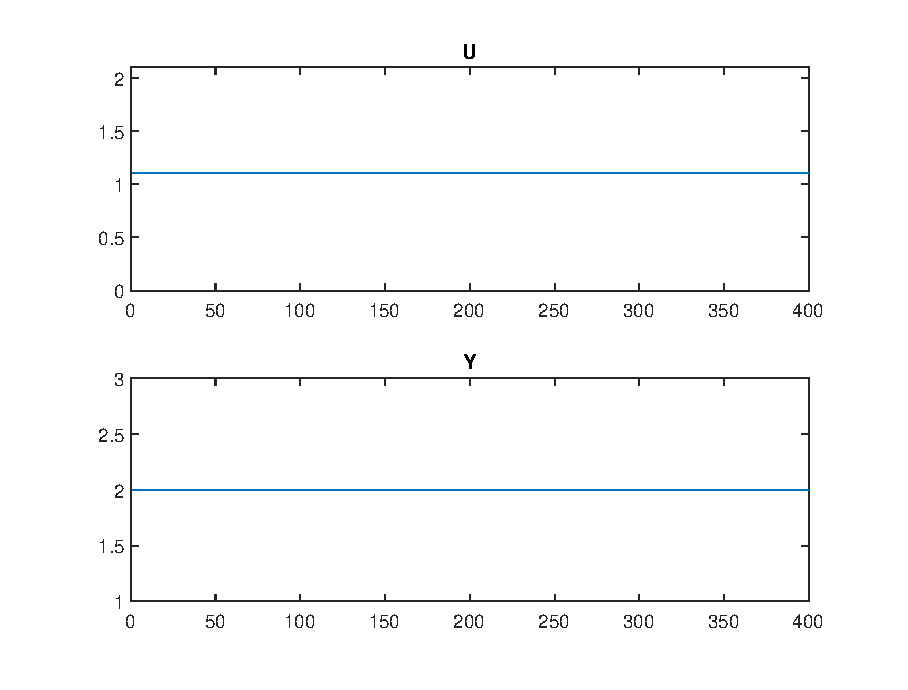
\includegraphics[scale=0.5]{rysunki/p1.eps}
\caption{Odpowied� skokowa dla algorytmu DMC}
\end{figure}

\section{Implementacja}
Implementacja fukcji wykorzystanych do wykonania zadania zawarte s� w skrypcie \verb+podpunkt_3_v1.m+.